\chapter{Theory of Clouds and Radiation}%("Theory of ...."?)
\label{chap:theory}
In this thesis the term shortwave (SW) refers to the wavelength band that carries most of the energy associated with solar radiation, including the visible spectrum and the shorter waves in the near infrared ($\lambda < 4\mu m$~\citep{Wallace2006}). Longwave (LW) refers to wavelengths emitted by the earth-atmosphere system (terrestrial radiation) including the longer waves in the near infra red and wavelengths in the infrared spectrum ($\lambda > 4\mu m$~\citep{Wallace2006}). 

In this chapter how cloud properties can influence radiation is presented, followed by a section on cloud effects on aerosols. Lastly a brief overview of clouds in the Arctic, with focus on stratus, is presented. 

\section{Cloud effects on radiation}
The cloud microphysical properties that determine the cloud radiative properties include: the amount of condensed water, the size and shape of the cloud particles, and if the particles are liquid or ice~\citep{Curry1996}.

\subsection{The Cloud -- a gray body}
Stefan–Boltzmanns law states that the flux density emitted by a blackbody is proportional to the fourth power of the absolute temperature~\citep{Liou2002}. 
\begin{equation}
F = \epsilon_{\lambda} \sigma T^4
\label{eqn:stefanboltzmann}
\end{equation}
where $\epsilon_{\lambda} = 1$ is the emissivity for a blackbody at wavelength $\lambda$. $F$ ($\text{W~m}^{-2}$) is the flux density emitted  by the body, and $\sigma = 5.67\cdot 10^{-8} \text{Jm}^{-2}\text{sec}^{-1}\text{K}^{-4}$ is the Stefan–Boltzmann constant. A blackbody both absorbs and emits at maximum, and the ratio of absorption and emission to the maximum is given by the absorptivity, $\alpha_{\lambda}$, and the emissivity, $\epsilon_{\lambda}$, for wavelength $\lambda$. Kirchoff's law states that the absorptivity and emissitivty for a medium are equal for each wavelength in the longer wavelength spectra: $\alpha_{\lambda} = \epsilon_{\lambda}$~\citep{Liou2002}. Kirchoff's law is only applicable for LW radiation at local thermodynamic equilibrium in the lower 60-70~km of the atmosphere. Since this study focuses on the lowest 2~km of the troposphere, the law is applicable.

A cloud can be defined as a a gray body, which means that $\alpha_{\lambda}$and $\epsilon_{\lambda}$ are not maximum, $\alpha_{\lambda}=\epsilon_{\lambda}<1$~\citep{Liou2002}.

The cloud LW emissivity, $\epsilon$, is a measure of the emittance of LW radiation by the cloud. From Stefan-Boltzmann's law, equation~\ref{eqn:stefanboltzmann}, the flux density emitted by a body depends on the body's temperature and it's emissivity. The cloud longwave emissivity is given by~\cite{Liou1992}
\begin{equation}
\epsilon = 1 - \exp(-k_v^c \text{LWP})
\label{eqn:epsilon_lw}
\end{equation}
where $k_v^c$ is the mass absorption coefficient of cloud particles, LWP is the liquid water path, which is the vertically integrated amount of water, and is further explained in section~\ref{sec:lwc}. Equation~\ref{eqn:stefanboltzmann} shows that if one assumes constant cloud temperature, the flux density emitted by the cloud increases with increasing $\epsilon$, which increases with increasing LWP. Name some typical values, and calculate F?@ Check also, values for $k_v c$!!@

\subsection{Cloud optical depth}
\label{sec:cloudoptdep}
Cloud optical depth (or cloud optical thickness), $\tau$, is a measure of the cumulative depletion that a beam of radiation directed straight downward (zenith angle $\theta = 0$) would experience in passing through a defined cloud layer. Of the incident SW radiation on a cloud with optical depth $\tau$, a fraction $e^{-\tau}$ is not scattered and is defined as the transmissivity of the cloud -- the radiation that is not absorbed or scattered in passing through the cloud~\citep{Wallace2006}. The remaining $1-e^{\tau}$ has been scattered one or more times in passing through the cloud layer. The cloud optical depth is given by~\citep{Twomey1977}
\begin{equation}
\tau = \int_0^h k_{E}dz = \pi \int_0^h \int_0^{\infty} r^2 Q_E(r/\lambda) n(r,z) dr dz
\end{equation}
at height z above cloud base for a cloud of depth $h$, containing $n(r)dr$ drops with radius in the interval ($r, r + dr$) per cubic centimeter ($\text{cm}^{-3}$). $Q_E(r/\lambda)$ is the extinction efficiency and $k_{E}$ is the extinction coefficient~\citep{Twomey1977}. The extinction efficiency is a measure of how well a particle removes the incident radiation, either by scattering or absorption. In the visible, for $\lambda<<r$, $Q_E\approx 2$ is a good approximation~\citep{Hobbs1993}, and we get the simpler expression
\begin{equation}
\tau = 2\pi N r_e^2 h
\label{eqn:cloudtau1}
\end{equation}
where it is assumed that the cloud droplet radius can be approximated by the effective radius, $r_e$.

\subsection{Cloud albedo}
%Clouds contribute the most to the planetary albedo~\citep{Twomey1974}. The cloud albedo is given by~\citep{Hobbs1993}
In section~\ref{sec:cloudoptdep} it was stated that the incident SW radiation on a cloud layer is either transmitted or scattered. The scattered radiation is scattered by single droplets, and the single-scattering albedo, $\overline{\omega}$, is the fraction of energy that is not absorbed in a single-scattering event, but scattered. $\overline{\omega}$ can to a good approximation be assumed equal to 1. Which means that the absorption of SW is negligible for cloud water, which supports that the SW radiation is either transmitted or scattered. When the single-scattering albedo is taken to unity, the albedo (or reflectance) of a cloud layer is given by~\citep{Hobbs1993}%\citep{Meador1980}
\begin{equation}
A = \frac{(1-g)\tau}{1+(1-g)\tau} = \frac{1-g}{\frac{1}{\tau}+(1-g)}
\label{eqn:cloudalbedo}
\end{equation}
The cloud albedo, $A$, is then a function of the SW optical depth of a cloud, $\tau$, and the asymmetry factor $g$. The asymmetry factor gives the direction of scattered radiation by the cloud, and is given by $g=\overline{\cos \theta}$ where $\theta$ is the scattering angle. $g$ is a power-averaged value of the cosine of the scattering angle~\citep{Twomey1974}. $g=1$ indicates pure forward scattering and $g=-1$ indicates pure back-scattering. According to Twomey, $g=0.8$ or $0.9$ for warm clouds, which means that most of the scattered energy is scattered forward.

%It is obvious from equations for $A$ and $\epsilon$ that a when $r_e$ is small - the albedo increases, and when it is larger the cloud albedo decreases. What about emissivity??

%How do clouds reflect radiation? What is the effect of more water? Or more ice? What about the droplet size? (effective radius)\\
%How do clouds absorb and emit radiation? Effect of more or less water or ice? Droplet size?    INCLUDE RADIATION EQUATION!

%Ice is more effective in reflecting SW than water. Snow has a higher albedo than rain. Is there any use in presenting some albedo values for water, snow, ice? Or open water versus sea ice? New ice versus old sea ice?

\subsection{Cloud droplet effective radius}
The cloud droplet effective radius determines important radiative properties of a cloud, cloud albedo ($A$) and cloud emissivity ($\epsilon$)~\citep{Hansen1974}, and is therefore of particular interest. 

The cloud droplet effective radius is a mean of the size distribution of cloud droplets, weighted by the droplet cross section. The effective radius, $r_e$, may be written
\begin{equation}
r_e = \frac{\int r^3 n(r) dr}{\int r^2 n(r) dr}
\label{eqn:re}
\end{equation}

It can be seen from equation~\ref{eqn:cloudtau1} that a decrease in $r_e$, when $N$ and $h$ is kept constant decreases the optical depth of the cloud. Whereas an increase in $r_e$ increases the cloud optical depth. It has already been established from equation~\ref{eqn:cloudalbedo} that a(n) decrease (increase) in the cloud optical depth leads to a(n) decrease (increase) in the cloud albedo $A$. The effect of $r_e$ on $\epsilon$ is through the LWP and is described in the following section.

\begin{figure}
\centering
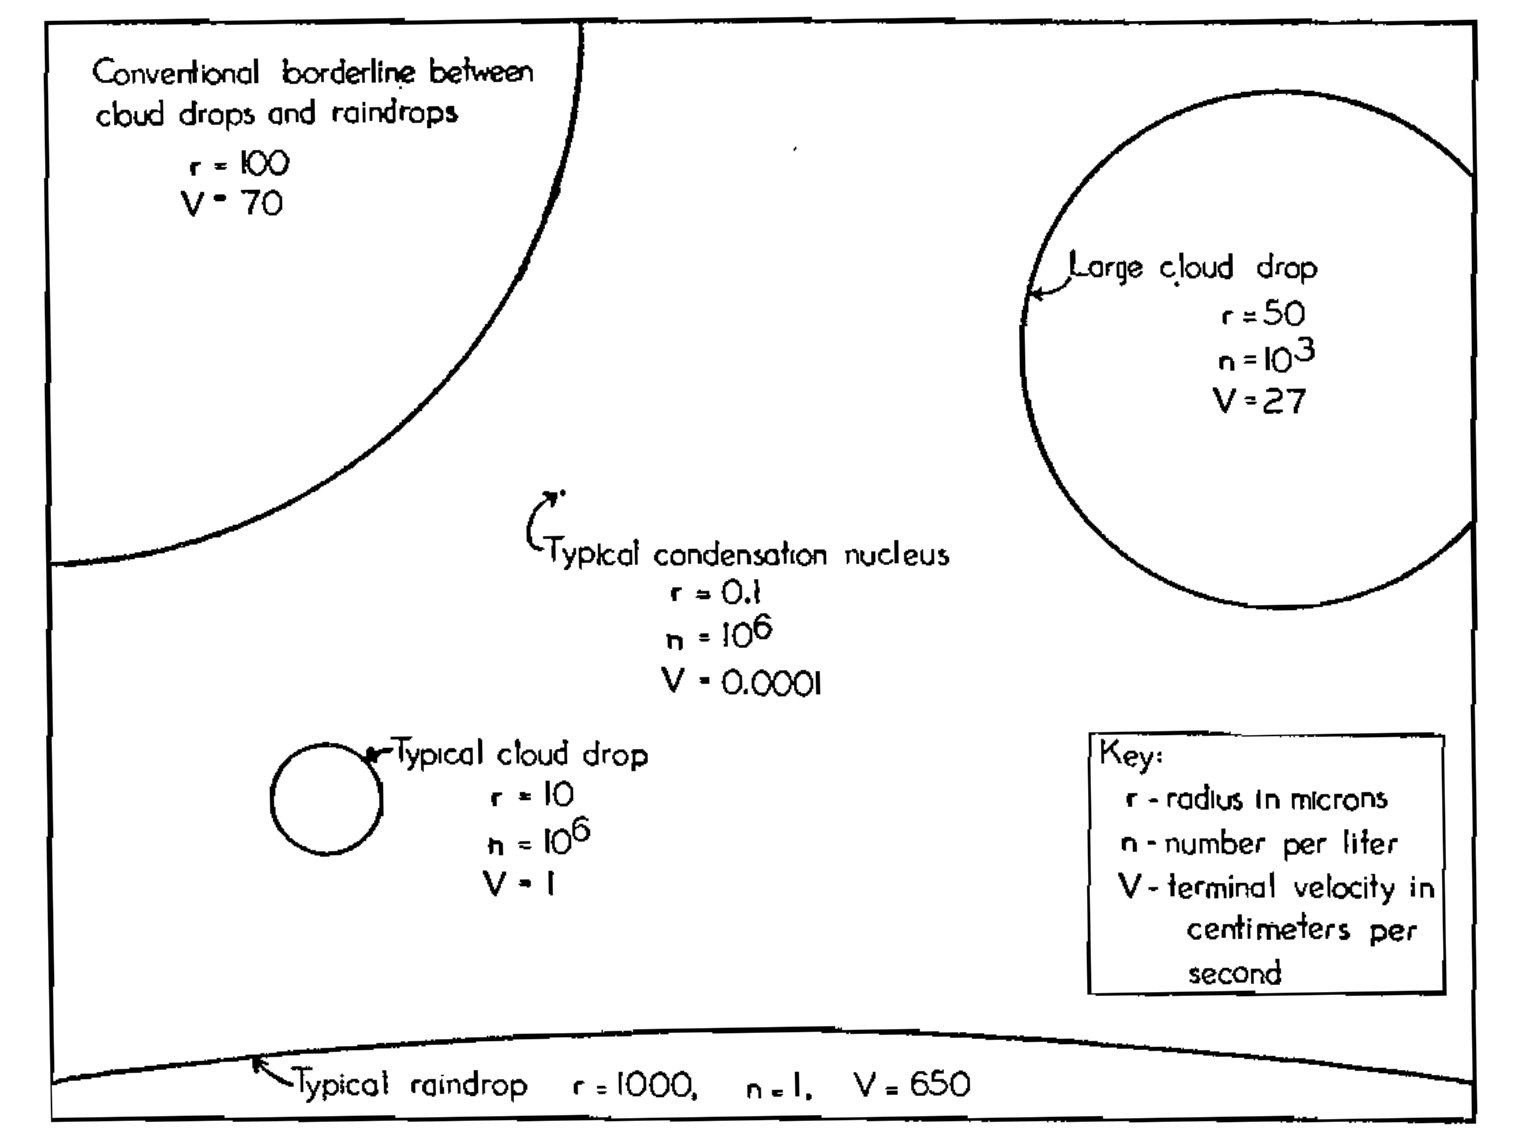
\includegraphics[width=0.85\textwidth]{theory/dropletsize.png}
\caption{Typical sizes of cloud condensation nuclei (CCN), cloud droplet, large cloud droplet, borderline between cloud droplet and raindrop and typical size of raindrop.% Adapted
 From~\citep{McDonald1958}.}
\label{fig:dropletsize}
\end{figure}
The effective radius is typically on the order of a few micro meters $\mu\text{m}$. Typical size of a cloud droplet is depicted in figure~\ref{fig:dropletsize}. The figure also includes typical sizes of cloud condensation nuclei (CCN), large droplet, borderline between cloud droplet and raindrop and typical size of a raindrop.


\subsection{Liquid water content and path}
\label{sec:lwc}
The amount of condensed water can be expressed by the liquid water content (LWC) in the cloud, often presented with units $\text{g~m}^{-3}$ and is proportional to the cloud droplet number concentration (CDNC), and cloud particle size. From~\citet{Rogers1989} the number of droplets with radius $r$ can be expressed by
\begin{equation}
N = \int n(r) dr
\end{equation}
where $N$ is the CDNC ($\text{cm}^{-3}$), and $n(r)$ is the number of droplets with radius $r$. If the radius is approximated to be the mean volume radius $\overline{r}$, the LWC for spherical droplets can be written
\begin{eqnarray}
\text{LWC} &=& \int \rho_l \frac{4}{3} \pi r^3 n(r) dr\\
&=& \frac{4}{3} \pi \rho_l \int r^3 n(r) dr\\
&=& \frac{4}{3} \pi \rho_l \overline{r}^3 \int n(r) dr\\
&=& \frac{4}{3} \pi \rho_l \overline{r}^3 N 
\end{eqnarray}
where the last equation shows the proportionality of LWC to the cloud droplet number concentration $N$, and to $\overline{r}$. $\rho_L$ is the density of liquid water. Knowing the effective radius from equation~\ref{eqn:re}, it is preferred to express the LWC as a function of that. The effective radius $r_e$ and $\overline{r}$ are related by
\begin{equation}
r_e = \kappa \overline{r}
\end{equation}
where $\kappa = 1.14$ for continental clouds and $\kappa = 1.08$ for maritime clouds~\citep{Martin1994}. $\kappa$ is close to unity and if it is simply taken to unity the LWC may be written
\begin{equation}
\text{LWC} = \pi \rho_l r_e^3 N
\label{eqn:LWC}
\end{equation}

Another common measure of condensed water is the liquid water path (LWP).
If the LWC is integrated over a column, from the base to the top, it gives the LWP of that column.
\begin{equation}
\text{LWP} = \int_{base}^{top} \text{LWC} dz
\end{equation}
The LWP is the column of liquid water in a cloud and is usually expressed in $\text{g~m}^{-2}$.

What effect a change in LWP has on incoming and outgoing radiation can be seen when the cloud optical depth is expressed as a function of LWP. Recall the cloud optical depth for SW radiation from equation~\ref{eqn:cloudtau1} and rewrite it to get the CDNC ($N$) on the left side
\begin{equation}
N = \frac{\tau}{2\pi r^2_e h}
\end{equation}
If the equation for LWC, equation~\ref{eqn:LWC}, is also rewritten to get $N$ on the left side, like so
\begin{equation}
N = \frac{3\text{LWC}}{4\pi \rho_l r^3_e}
\end{equation}
the cloud optical depth in the visible ($\tau$) can be written as a function of LWP and $r_e$:
\begin{eqnarray}
\frac{\tau}{2\pi r^2_e h} &=& \frac{3\text{LWC}}{4\pi \rho_l r^3_e}\\
\tau &=& \frac{2\pi r^2_3 h 3\text{LWC}}{4\pi \rho_l r^3_e}\\
\tau &=& \frac{3\text{LWC} h}{2\rho_l r_e}\\
\tau &=& \frac{3\text{LWP}}{2\rho_l r_e}
\label{eqn:cloudtau}
\end{eqnarray}
Where $\text{ LWC }h \approx \text{LWP}$. It is now clear that, if the droplet size is constant, an increase in the LWP increases the optical depth of a cloud, $\tau$. An increase in $\tau$ would make the denominator in equation~\ref{eqn:cloudalbedo} for the cloud albedo, $A$, smaller and thereby increase the cloud albedo. An increase in $A$ also means a reduction in SW radiation reaching the surface. In that way, an increase in LWP would have a cooling effect on the surface.
But, the LW radiation must also be considered. A change in LWP changes the cloud emissivity. Equation~\ref{eqn:epsilon_lw} shows that $\epsilon$ increases (decreases) with increasing (decreasing) LWP. Meaning that and increase in LWP would increase the flux density emitted by the cloud, following Stefan-Boltzmann's law from equation~\ref{eqn:stefanboltzmann}, and have a warming effect on the surface. Thus, a change in LWP gives opposite effects warming for shorter and longer wavelengths.

\begin{figure}
\centering
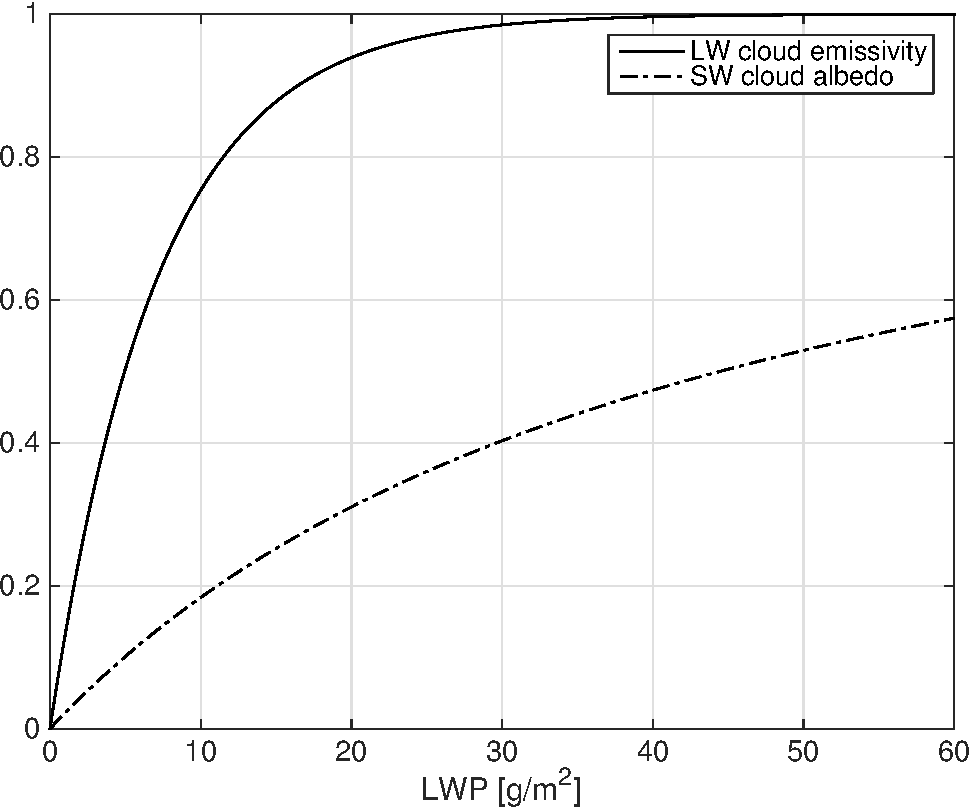
\includegraphics[width=0.6\textwidth]{theory/eps_alb.pdf}
\caption{Cloud LW emissivity and SW albedo as a function of liquid water path (LWP), for clouds containing no ice.}
\label{fig:epsalb}
\end{figure}

In figure~\ref{fig:epsalb} both SW cloud albedo, $A$, and the LW cloud emissivity, $\epsilon$, are shown as functions of the LWP for ice-free clouds. It is based on equations~\ref{eqn:epsilon_lw},~\ref{eqn:cloudalbedo} and~\ref{eqn:cloudtau}, where $k_v^c=0.14$, $g=0.85$, $\rho_l=1000\text{kg/m}^3$ and $r_e = 10\mu\text{m}$ which is a typical cloud droplet radius according to figure~\ref{fig:dropletsize}. A cloud emissivity less than unity is mainly a consequence of low LWP, as it is saturated in the LW already at a LWP of 40 to 45 $\text{g/m}^2$. A further increase in LWP does not increase the LW emission by the cloud and hence not the downward LW at the surface, but it does on the other hand still increase the cloud albedo. The increase in reflected SW radiation with LWP would thus work to even out the effect of emission of LW to the ground. 

\subsection{Ice water path}
 Clouds also consist of ice, not just liquid water. The amount of ice in a cloud for a given ice crystal size distribution is given by the ice water content (IWC)~\cite{Liou2002}
\begin{equation}
\text{IWC} = \int V \rho_i n(L)dL
\end{equation}
where $L$ is the maximum dimension of an ice crystal, $V$ is the volume, $\rho_i$ is the density of ice and $n(L)$ is the ice-crystal size distribution. As for the water droplets the cloud optical depth, $\tau$, and mean effective crystal size, $D_e$, are related through
\begin{equation}
\tau \approx \text{IWP}(c + b/D_e)
\label{eqn:icetau}
\end{equation}
where IWP denotes the ice water path $\text{IWP} = \text{IWC} \cdot h$ for a layer of thickness h, and $c \approx -6.656 \times 10^{-3}$ and $b \approx 3.686$ for ice columns~\citep{Liou2002}. Equation\ref{eqn:icetau} clearly shows that an increase in the IWP increases the cloud optical depth (when $D_e$ is kept constant), which in turn, according to equation\ref{eqn:cloudalbedo}, increases the cloud albedo. The opposite is obvious for $D_e$; when $D_e$ increases, the optical depth decreases, provided the IWP is unchanged, which in turn decreases $A$.

\section{Aerosols and clouds}
Aerosols have a direct effect on the climate by scattering and absorbing SW radiation, and scattering, absorbing and emitting LW radiation. A small subset of the atmospheric aerosols also serve as particles which water vapor can condense on to form droplets~\citep{Wallace2006}. Aerosols upon which water vapor can condense are called cloud condensation nuclei (CCN). Typical size for CCN is shown in figure~\ref{fig:dropletsize}. For low temperatures ($\sim$-20 to -5$\degree$C)~\citep{Wallace2006}, a few aerosols act as ice nuclei (IN) which if present allow for cloud ice to form. With IN cloud ice can form through heterogeneous freezing, contact nucleation and deposition~\citep{Wallace2006}. Heterogeneous freezing is when a droplet already contains a freezing nucleus and is brought to lower temperatures so that the already condensed water on the particle freezes. Contact nucleation is when a supercooled droplet (droplet with temperature below 0$\degree$C) is hit by a suitable ice nucleus, and deposition is when water vapor freezes directly on the nucleus.

Some typical CCN are sulfates, sea salt and organic carbon, whereas IN are typically mineral dust, and are all included in the model used in this study~\citep{Thompson2014}, which is described in the next chapter. Typical aerosol number concentrations are 10$^3$ to 10$^5$~$\text{cm}^{-3}$, the number of those that can act as CCN range from 10$^{-2}$ to 10$^3$~$\text{cm}^{-3}$, and the number if available IN is about 10$^{-3}~\text{cm}^{-3}$. Through clouds these aerosols that act as CCN or IN also have an indirect effect. The amount of CCN and IN available affect the properties of the clouds. There are two known indirect effects that aerosols have on climate, through clouds.
 
\subsection{The first indirect effect}
The first indirect effect was proposed by~\citet{Twomey1974} and is often referred to as the Twomey effect. It describes the enhancement of cloud albedo as a consequence of an increase in aerosol content and thereby available CCN.

If there are few CCN in an area, a cloud formed there would be a clean cloud with few, but large droplets and therefore have a low albedo. If the area had high aerosol concentration, the cloud would be polluted and have more numerous but smaller droplet, provided the LWP is the same, which means it would have a higher optical depth in the SW according to equation~\ref{eqn:cloudtau}, which through equation~\ref{eqn:cloudalbedo} gives a higher albedo.

The increase in cloud albedo due to pollution is shown in the left-most 4 figures in figure~\ref{fig:indirecteffects}. The figure shows that with more CCN available, in a polluted environment, the cloud or cloud layer, appears brigther than when the air is clean (fewer available CCN).

\begin{figure}
\centering
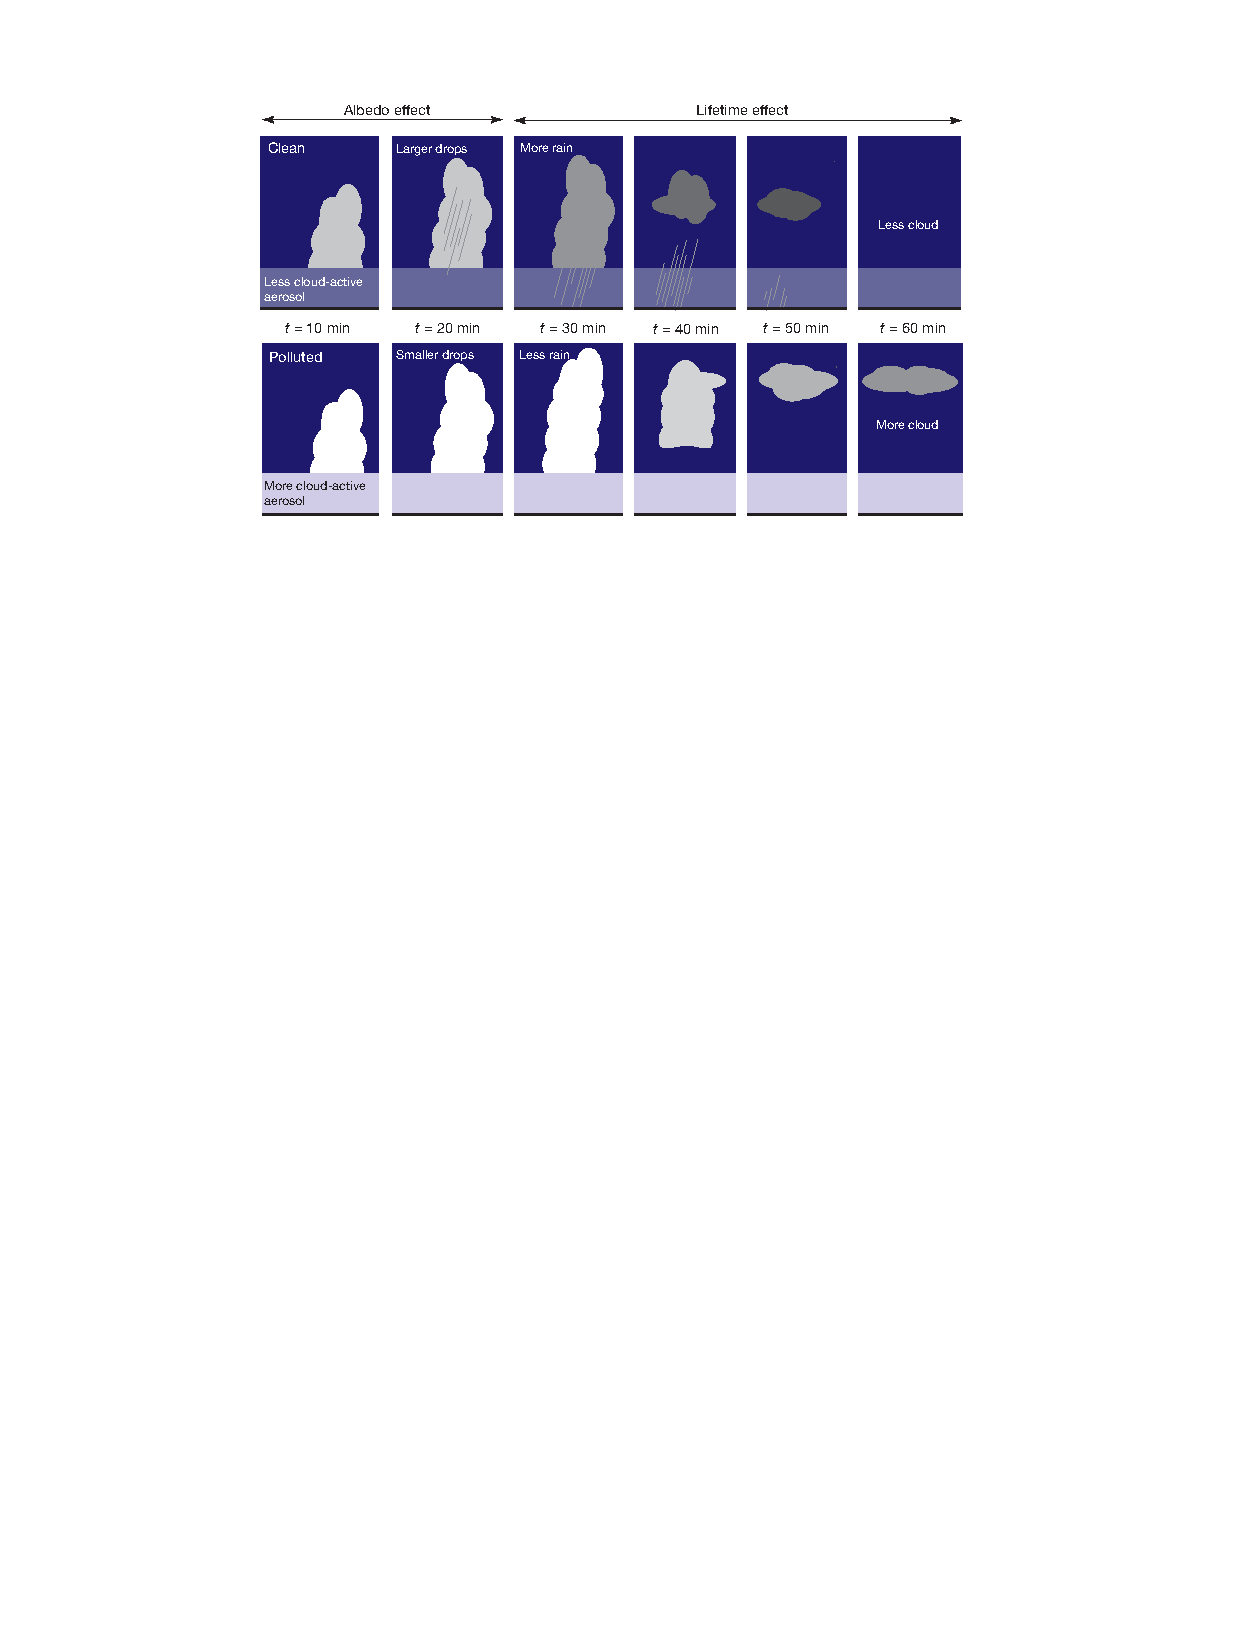
\includegraphics[width=1.1\textwidth]{theory/indirecteffects.pdf}
\caption{Figure showing the first indirect effect (albedo effect) to the left and the second indirect effect (lifetime effect) to the right. The figure includes a time axis to show the time scale of a precipitation process. The upper and lower panel show the clean and polluted case respectively. The figure is taken from~\cite{Stevens2009}.}
\label{fig:indirecteffects}
\end{figure}

Equation~\ref{eqn:cloudtau1} shows that, if the effective radius is kept constant, the cloud optical depth will change with changes in CDNC ($N$ in the equation). The CDNC is affected by the number of available CCN, and as the aerosol number concentration changes so will the number of CCN, and hence the CDNC and optical depth. Furthermore if a cloud has many small droplets, the cloud optical depth will be higher. Whereas fewer cloud droplets will yield a lower optical depth, provided $r_e$ is kept constant, resulting in more SW radiation reaching the ground. The same is clear for ice, from equation~\ref{eqn:icetau}, where it was shown that a larger ice crystal size yields a lower albedo, provided the IWP is unchanged. Thus the first indirect effect also applies to ice, since a decrease in $D_e$, while IWP is kept constant, means an increase in particle number, but a decrease in particle size and hence an increase in $\tau$ which in turn increases the cloud albedo.

\subsection{The second indirect effect}
The second indirect effect was proposed by~\citet{Albrecht1989}, and is also known as the lifetime effect.

The second indirect effect suggests more numerous but smaller droplets reduce the precipitation efficiency and by that enhances the cloud lifetime and hence the cloud reflectivity~\citep{Albrecht1989}. The effect is depicted in figure~\ref{fig:indirecteffects} as the lifetime effect, where it is shown that in the lower panel, the polluted case, the cloud does not precipitate and is therefore still present after an hour, where as the cloud in the upper panel, the clean case, is gone due precipitation.

Figure~\ref{fig:dropletsize} shows that droplets have to grow to a size of typically 1000$\mu\text{m}$ for precipitation to form. A rain drop is formed when smaller droplets collide and coalesce into a larger droplet, which also falls to collect smaller droplets until it is large enough to fall out of a cloud as precipitation. The second indirect effect suggests that an increase in aerosol burden leads to the water vapor being spread over a higher number of droplets, giving them a smaller effective radius which will prohibit them from growing to a raindrop. The hypothesis is that if the cloud does not precipitate, it will grow denser and live longer since the cloud water is not removed by precipitation. According to~\citet{Lohmann2005} this effect had been estimated to be of the same order as the first indirect effect. It has since been shown that the effect is in fact small globally averaged~\citep{Stevens2009}. \citet{Stevens2009} state that in the cases where an increased aerosol burden prohibits precipitation, the cloud can be entrained by dryer air which leads to evaporation of the cloud droplets, and the cloud ceases to exist. On the other hand, an increase in aerosol burden in deep precipitating clouds may lead to more, not less precipitation~\citep{Stevens2008}.

%Production of DMS by phytoplankton Charlson 1987....
%-------- Droppe dette?
%\subsection{Cloud effects on aerosols}
%Cloud presence is due to water vapor condensing on CCNs and possibly freezing if the aerosol's structure resembles that of an ice crystal, IN. Processes known to affect the local aerosol concentration are: precipitation because the precipitation will wash out aerosols from the air when falling through it, this is also known as scavenging. Pollution, increases in aerosol concentration might inhibit precipitation and cause longer-lived, more persistent clouds, which will in turn affect the radiation balance.

%Not only the aerosol burden is important, if it is the same for two areas with different meteorological forcing that would also affect the cloud properties. Say an area has a weaker updraft than another area, a cloud formed due to the weaker updraft will have lower LWC, lower albedo and little precipitation. The cloud formed in a stronger updraft will have higher LWC, higher albedo and be more precipitating.
%--------

\section{Arctic stratus}
% Move to introduction: The Arctic cloud cover is dominated by low clouds~\citep{Klein1993}.
% New try!
Clouds in the Arctic differ from clouds elsewhere in that they have a net warming effect, as opposed to the global mean net cooling effect~\citep{Shupe2004}. Winter in the Arctic (polar night) is completely dark and free of incoming SW radiation. The Arctic summer on the other hand has sunlight 24/7. The amount of solar radiation reaching the surface is limited by the optical depth of the atmosphere it passes through. The normal optical depth is a measure of the cumulative depletion of a radiation beam directed straight downward (zenith angle $\theta = 0$) from the top of the atmosphere to a level $z$, defined by~\citep{Wallace2006}
\begin{equation}
\tau_{norm} = \int_z^\infty k_{\lambda} \rho_a R dz
\end{equation}
where $k_{\lambda}$ is the mass absorption coefficient, $\rho_a$ is the density of air and $R$ is the mass of absorbing gas per unit mass of air.  The undepleted fraction of the radiation is given by the transmissivity, $T_{\lambda}$, of the layer. The transmissivity depends on the normal optical depth and the angle at which the beam deviates from straight down, the zenith angle $\theta$. The transmissivity is defined by~\citep{Wallace2006}
\begin{equation}
T_{\lambda} = e^{-\tau_{norm} \sec \theta}
\end{equation}
It is obvious that $T_{\lambda}$ decreases with increasing $\theta$. Since the Arctic is far North, the incoming solar radiation is at a high zenith angle, and less SW reaches the surface than at lower latitudes. Consequently the SW reaching the surface in the Arctic is low compared to lower latitudes. Low clouds have a net cooling effect globally, due to their high albedo. In section~\ref{sec:cloudrad} it was shown that clouds not only reflect SW radiation, but also emit LW radiation. When there is little SW to reflect, the warming effect of the emission of LW radiation is enhanced.



Clouds in the Arctic are mostly optically thin and low lying~\citep{Curry1996}.


%-------
The clouds studied in this thesis are low (up to about 1600~m) stratus clouds, in the Arctic. Stratus clouds are low layered clouds that form when extensive areas of stable air is lifted. They are normally between 0.5 and 1~km thick, and can be several km wide~\citep{Aguado2010}. The largest amounts of low stratus clouds in the Arctic are over the ocean~\citep{Klein1993}.
%The Arctic is the only region where the season of maximum stratus does not correspond to the season of greatest lower troposphere static stability~\citep{Klein1993}, which could be due to lack of evaporation during the cold winter months.
According to~\citet{Klein1993} stratus in the Arctic basin peaks during summer at nearly 62\%, while during the winter season the stratus only accounts for 18\% of the cloud cover. This leads them to conclude that the seasonal cycle of stratus in the Arctic is driven by the temperature cycle, thereby moisture content in the atmosphere, rather than the static stability.
%(, as opposed to other areas.)
%Low clouds have bases below 2000~m. Stratus (St) are layered clouds that form when extensive areas of stable air are lifted. Stratus clouds are normally between 0.5 and 1~km thick, whereas they can be several km wide~\citep{Aguado2010}.

As mentioned in Chapter~\ref{chap:introduction} there is no solar radiation to reflect during winter and the polar night in the Arctic, whereas in the summer the zenith angle is so high that even though there is sunlight 24 hours a day the cooling effect in summer does not average out the heating effect the clouds have in winter. A high zenith angle, means that the radiation has to travel through more atmosphere, which gives a higher optical depth and stronger depletion of the radiation beam. Consequently, the low clouds' ability to absorb and emit terrestrial radiation dominates over their reflective effect on the solar radiation.

%Are there any typical cloud properties special to the arctic? CURRY!
%Are they typically warm or cold clouds? And what does that mean?? Wallace2006 can help :)

The stratus clouds in the Arctic are typically thin (check with Curry@).
The air in the Arctic is very stable in winter (polar night), and clean since there are not many sources for pollution. In Autumn the sea ice extent reaches a minimum after the summer melt and leaves open water to influence low clouds and their properties. Some of the cloud radiative properties  are presented in the next section.

The tools and methods used to study Arctic clouds in this thesis are described in the following chapter.